%%%%%%%%%%%%%%%%%%%%%%%%%%%%%%%%%%%%%%%%%%%%%%%%%%%%%%%%%%%%%%%%%%%%%%%%
% This is the introduction chapter file.
%%%%%%%%%%%%%%%%%%%%%%%%%%%%%%%%%%%%%%%%%%%%%%%%%%%%%%%%%%%%%%%%%%%%%%%%
%
% Author:   René Widmer
%           Institute for Surgical Technology and Biomechanics ISTB
%           University of Bern
%           rene.widmer@istb.unibe.ch
%
% Date:     10/28/2009
%
%%%%%%%%%%%%%%%%%%%%%%%%%%%%%%%%%%%%%%%%%%%%%%%%%%%%%%%%%%%%%%%%%%%%%%%%

\chapter{Introduction}
% \section{Motivation}
The liver is an important organ in the human body that is often affected by
cancer. Untreated liver
cancer leads to death and the only curative treatment of it is surgery. Liver
resection surgery is the gold standard treatment and intraoperative ultrasound is the
tool used to navigate during these surgeries because it allowes to look into the
organ which helps to navigate. However, computer assisted navigation is not used regularly in
this kind of surgery
although it has the potential to improve
surgical outcome through increased precision, accuracy and reproducibility.

Conventional approaches create a virtual 3D model of the liver from medical
image data prior to the surgery. These models can then be used to plan the
resection surgery and to navigate during the intervention. Image to patient
registration is the task of aligning the virtal 3D model to the patients anatomy
in the operating room. In order to register, part of the patient's liver is
reconstructed intraoperatively to know the actual orientation and position of
the organ. Because the liver deforms between the preoperative imaging
and the surgery, a rigid registration can not superimpose the virtual and real
liver perfectly. To compensate for such deformations is a difficult and usolved
problem today.

Conventional approaches already reconstruct parts of the liver but they use them
for registration instead of navigation. This project focuses on the conceptualization, implementation and evaluation of a concept for the creation of an
intraoperative 3D model of the liver and the intraoperative resection planning
on such a model. Like this, the problems of registration and deformation
compensation would not need to be solved any more.  
% time used to  of the
% liver.
% Moreover, most navigation models are expensive and time-consuming.

% The goal of computer assisted surgeries is to reduce the time used to do the
% surgery and to also improve the surgical result for the patient.

% The accuracy of such navigation systems is affected by
% deformations of the liver during the surgery \cite{clements2017deformation}.


\section{The Liver} 
\subsection{Liver Anatomy}
The human liver overlies the gallbladder, is located in the right upper quadrant of the abdomen and has
different functions. It produces biochemicals necessary for digestion,
synthesizes proteins and detoxifies various metabolites. A human liver wheighs
normally around 1.5 kg, is the heaviest internal organ and the largest gland
of the human body. Two large blood vessels are connected to the liver: the
portal vein and the hepatic vein. Both of them subdivide into small
capillaries called \textit{liver sinusoids} and then lead to the functional
units of the liver known as \textit{lobules}. To refer to the different parts of
the liver, it is subdivided into eight segments (Figure \ref{fig:liverSegments}). Each segment has its own
vascular inflow and outflow.
\begin{figure}[H]
  \centering
 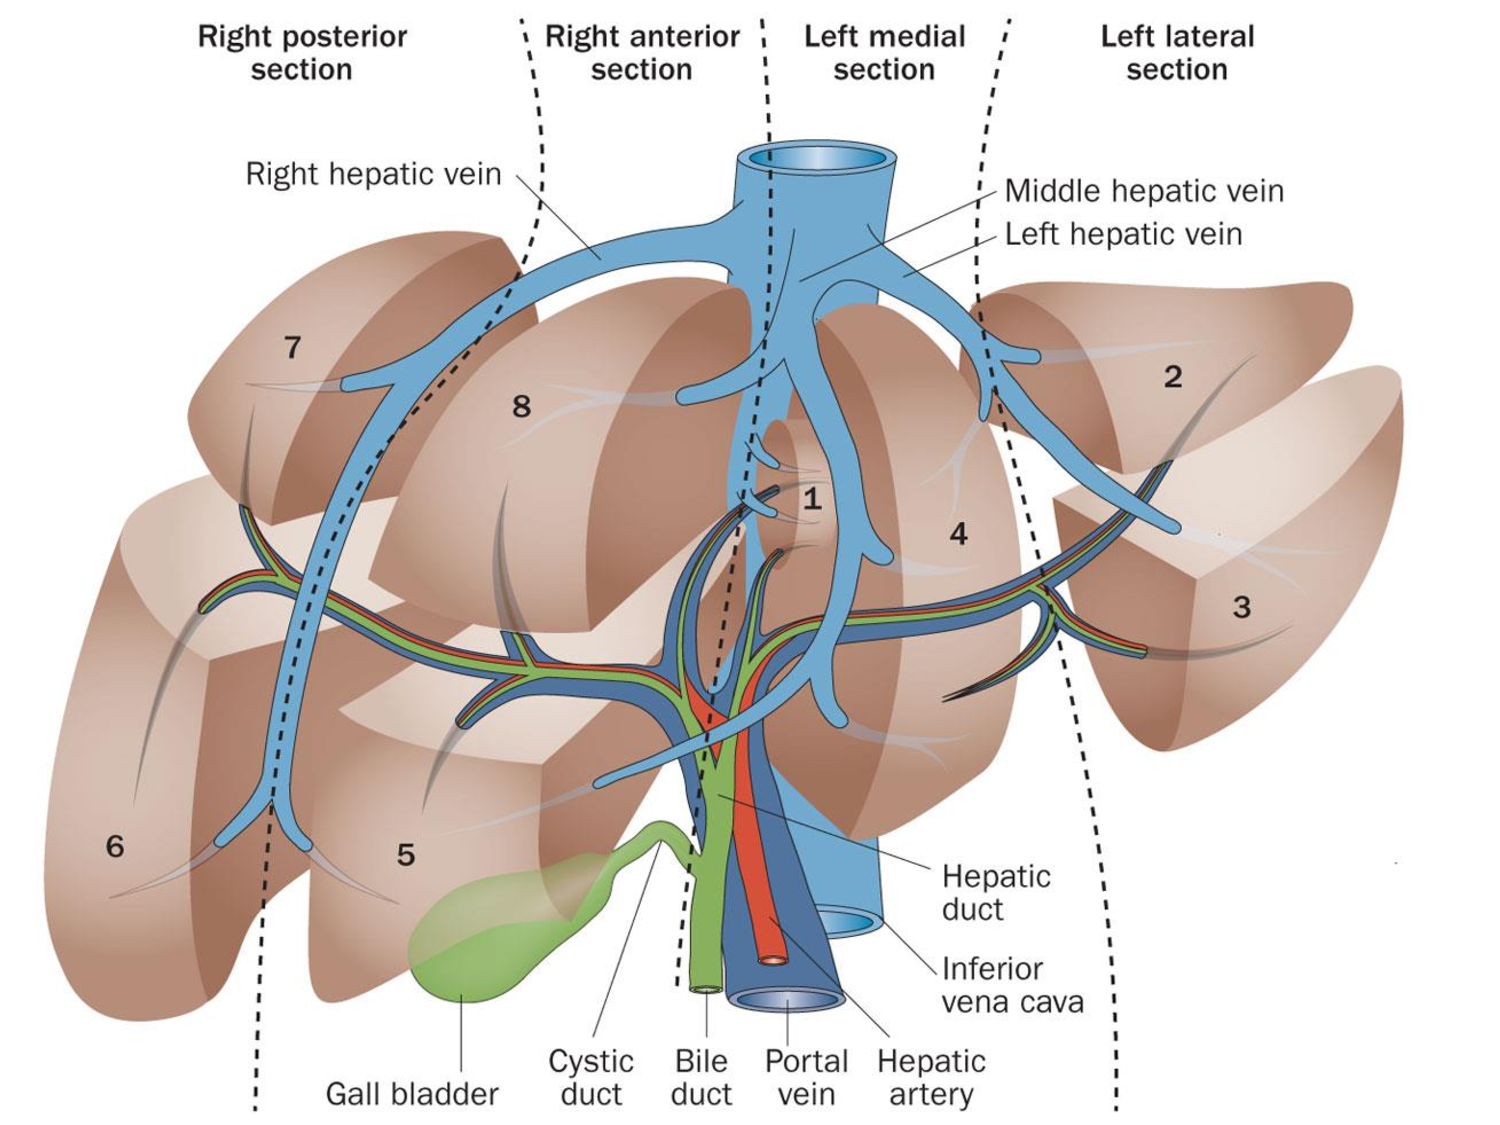
\includegraphics[width=\textwidth]{liverSegments}
  \caption{The liver and its eight Chouinaud segments. In red is the hepatic
    artery which transports blood from the heart a into the liver. In dark blue
    the portal vein, it transports blood from the gut into the liver. All the
    blood leavs the liver through the hepatic veins to the vena cava \cite{siriwardena2014management}.}
  \label{fig:liverSegments}
\end{figure}

\subsection{Liver Cancer}
% \textcolor{green}{Liver metastatis are more common in US/Europe, in asia it's the other way around for example}
Liver cancer is cancer that starts in the liver. If the cancer has spread from
elsewhere to the liver, then it is known as liver metastasis. Liver metastasis
are about 20 times more common in the United States and in Europe than primary tumors. One of the reasons for that
is the rich blood supply of the liver which helps the tumors to grow
\cite{mcguire2016world}. In asia it's the other way round, more people suffer
from liver cancer than from liver metastases. Liver cancer patients often have chronic liver diseases
such as cirrhosis, problems of alcohol abuse, and viral hepatitis (B or C)
\cite{galun2015hepatocellular}. The gold standard to treat liver cancer are
surgical resections \cite{lencioni2012local}. The liver tissue can easily regrow, given that after resection there is
enough healthy tissue and blood supply preserved. Alternatively to resections
one can treat liver tumors by local ablation. Both variants treat the tumors
with a safety margin of 10 mm. This safety margin ensures that all tumor cells
are destroyed and to prevent further spread of cancer cells \cite{mahnken2009ct}.
\section{Liver Resections} 
% \textcolor{green}{explain liver resections a bit more in detail, also what instruments are used and what to do with a blood vessel}
Hepatectomy is the surgical resection (removal of all or part) of the liver.
Liver resections are considered major surgeries and are done under general
anesthesia. If no other internal organs of the body are affected and the liver
is not cirrhotic, then 70\% to 80\% of the total liver volume can be removed in a
surgical resection. For patients with cirrhotic livers, not more than 50\% of
the total liver volume should be removed \cite{pianka2011liver}. Liver tissue is
cut using instruments like the BiClamp® vessel-sealing device (Figure \ref{fig:BiClampExplained}). Such devices can
simultaneously transect liver parenchyma and seal vessels with diameters smaller
than 7 mm \cite{zhao2017biclamp}. For larger vessels, resorbable clamps are used
to prevent heavy bleeding. Most hepatectomies are done laparoscopicly. However for complicated
cases also open surgeries are done \cite{cherqui2000laparoscopic}.
\begin{figure}[H]
  \centering
  \minipage{0.32\linewidth}
  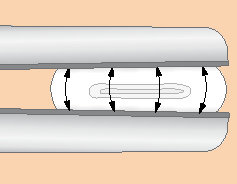
\includegraphics[width=\linewidth]{BiClamp1}
  \endminipage
  \hfill
  \minipage{0.32\linewidth}
  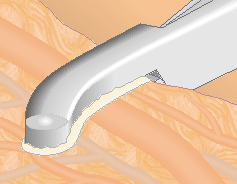
\includegraphics[width=\linewidth]{BiClamp2}
  \endminipage
  \hfill
  \minipage{0.32\linewidth}
  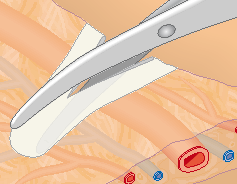
\includegraphics[width=\linewidth]{BiClamp3}
  \endminipage
  \hfill 
 \caption{A vessel sealing device is used to transect liver parenchyma and split
   blood vessels then seal them so that no blood is lost. From left to right:
   First, the vessel is pressed together and then the tissue coagulated using a bipolar
   electrosurgical current. In some cases this is done twice. Finally the tissue
   is separated mechanically at the center of the visible coagulation area \cite{biClampPdfWithImages}. }
  \label{fig:BiClampExplained}
\end{figure}

Two resection techniques can be separated. Anatomical or parenchymal-sparing
resections (Figure \ref{fig:resectionsPlanning}). Most studies analyzing
long-term oncological outcomes have shown that there is no significant benefit
of anatomical resections over parenchymal-sparing ones in terms of 5-year overall
survival and disease-free survival. In anatomical resections
(Figure \ref{fig:resectionsPlanning} A1) the tumors are removed by cutting along
anatomical vessel landmarks whereas in parenchymal-sparing resections (Figure
\ref{fig:resectionsPlanning} A2) only the tumor and surounding tissue is removed
such that the safety margin is respected. Parenchymal-sparing resections are
shown to be associated with less surgical stress, less postoperative
complications and higher feasibility of future resections. This work will concentrate on the parenchymal-sparing technique. 
\begin{figure}[H]
  \centering
 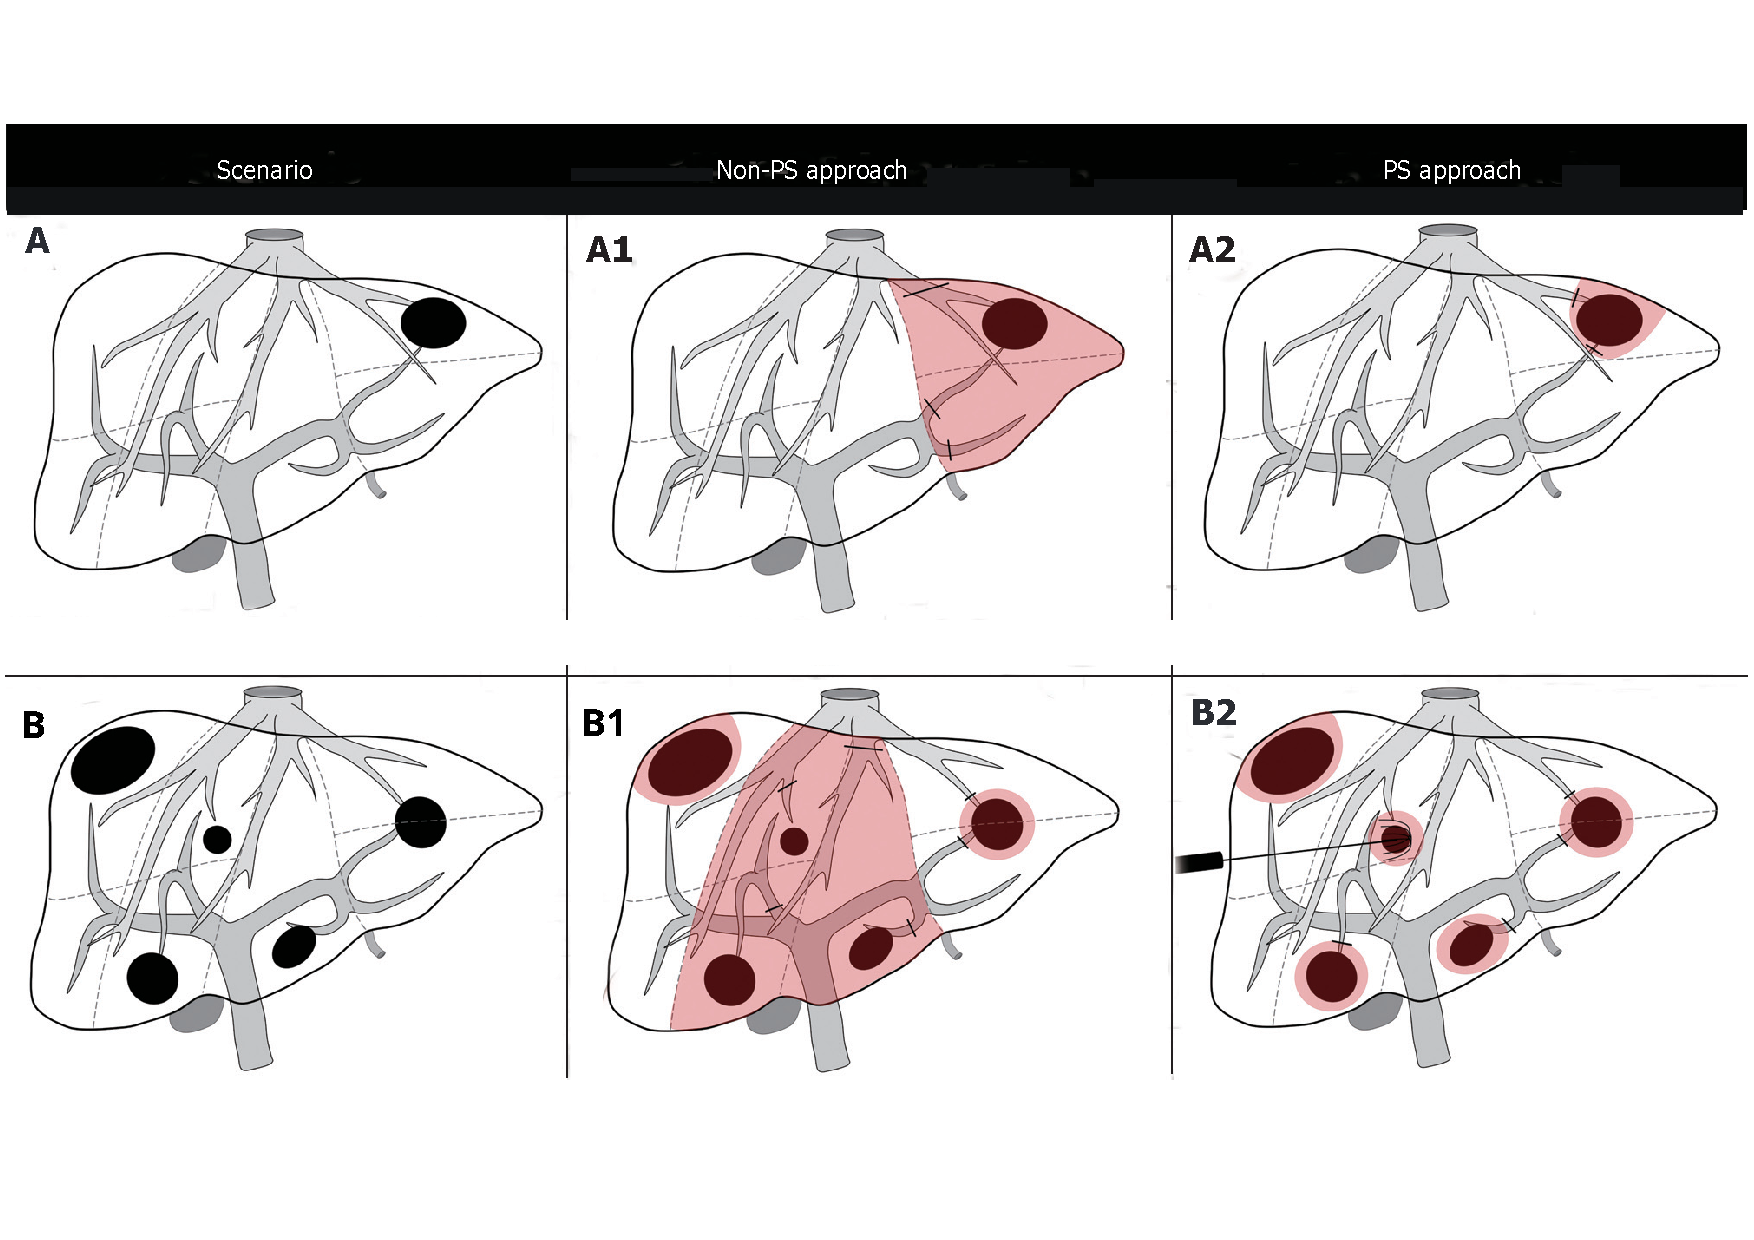
\includegraphics[width=\textwidth]{resectionsPlanning}
  \caption{Two different approaches to resect liver tumors in two different
    situations. The \textit{Scenario} column shows the situation of the
    patient's liver, the \textit{Non-PS approach} column shows how an anatomical
  resection plan would look like and the \textit{PS approach} column shows how a
parenchymal-sparing resection plan would look like \cite{alvarez2016parenchymal}.}
  \label{fig:resectionsPlanning}
\end{figure}


\paragraph{Parenchymal-sparing liver surgeries}
Resection is the established gold-standard treatment for liver tumors in
general. The surgical treatment of liver tumors has changed with the expansion of the
parenchymal-sparing liver resection technique. This technique involves preserving healthy
functional liver parenchyma by performing a wide range of liver resections. In
order to perform the appropriate type of resection, the site and
relationships of the tumor with glissonian pedicles or hepatic veins have to be
known.
For that reason, it is obvious that only the heavy use of intraoperative 
ultrasound makes it possible to perform parenchymal-sparing liver resections.
Parenchymal-sparing resections are preferably done laproscopic. This method is backed by technical, oncological,
and pathological arguments.
This approach has multiple benefits: decreases postoperative mortality and
morbidity rates, while preserving the function of the liver. In turn, the risk
of liver dysfunction is reduced and the possibility of re-resection in case of
reccurence increases. Overall, laparoscopic parenchymal-sparing liver surgeries offer
similar survival results compared to open ones \cite{Ferrero2017}.
%\cite{alvarez2016parenchymal}
% \section{Objectives} 
% The objectives of this Master's thesis are:
% \begin{itemize}
%   \item Implementation of the concept for an intraoperative 3D reconstrction
%   technique of the liver from intraoperative ultrasound. 
%   \item Implementation of the intraoperative resection planning.
% \end{itemize}
% This work focuses on open surgical procedures of liver hepatectomies and
% especially parenchymal-sparing methods.


%Laparoscopic anatomical hepatectomy (LAH)

\section{Intraoperative ultrasound}
% \textcolor{green}{Start with why US is used, then describe how it works and the limitations. from there you should have a nice transition to navigation}
In liver surgeries an intraoperative ultrasound device is used for intraoperative planning and
guidance inside the liver. It is used to locate tumors that are not
visible on the liver surface and to estimate their sizes from the ultrasound image. Figure \ref{fig:liverUS} shows an example of an
ultrasound image of the liver and its corresponding position in the 3D liver
model.

\begin{figure}[H]
  \centering
 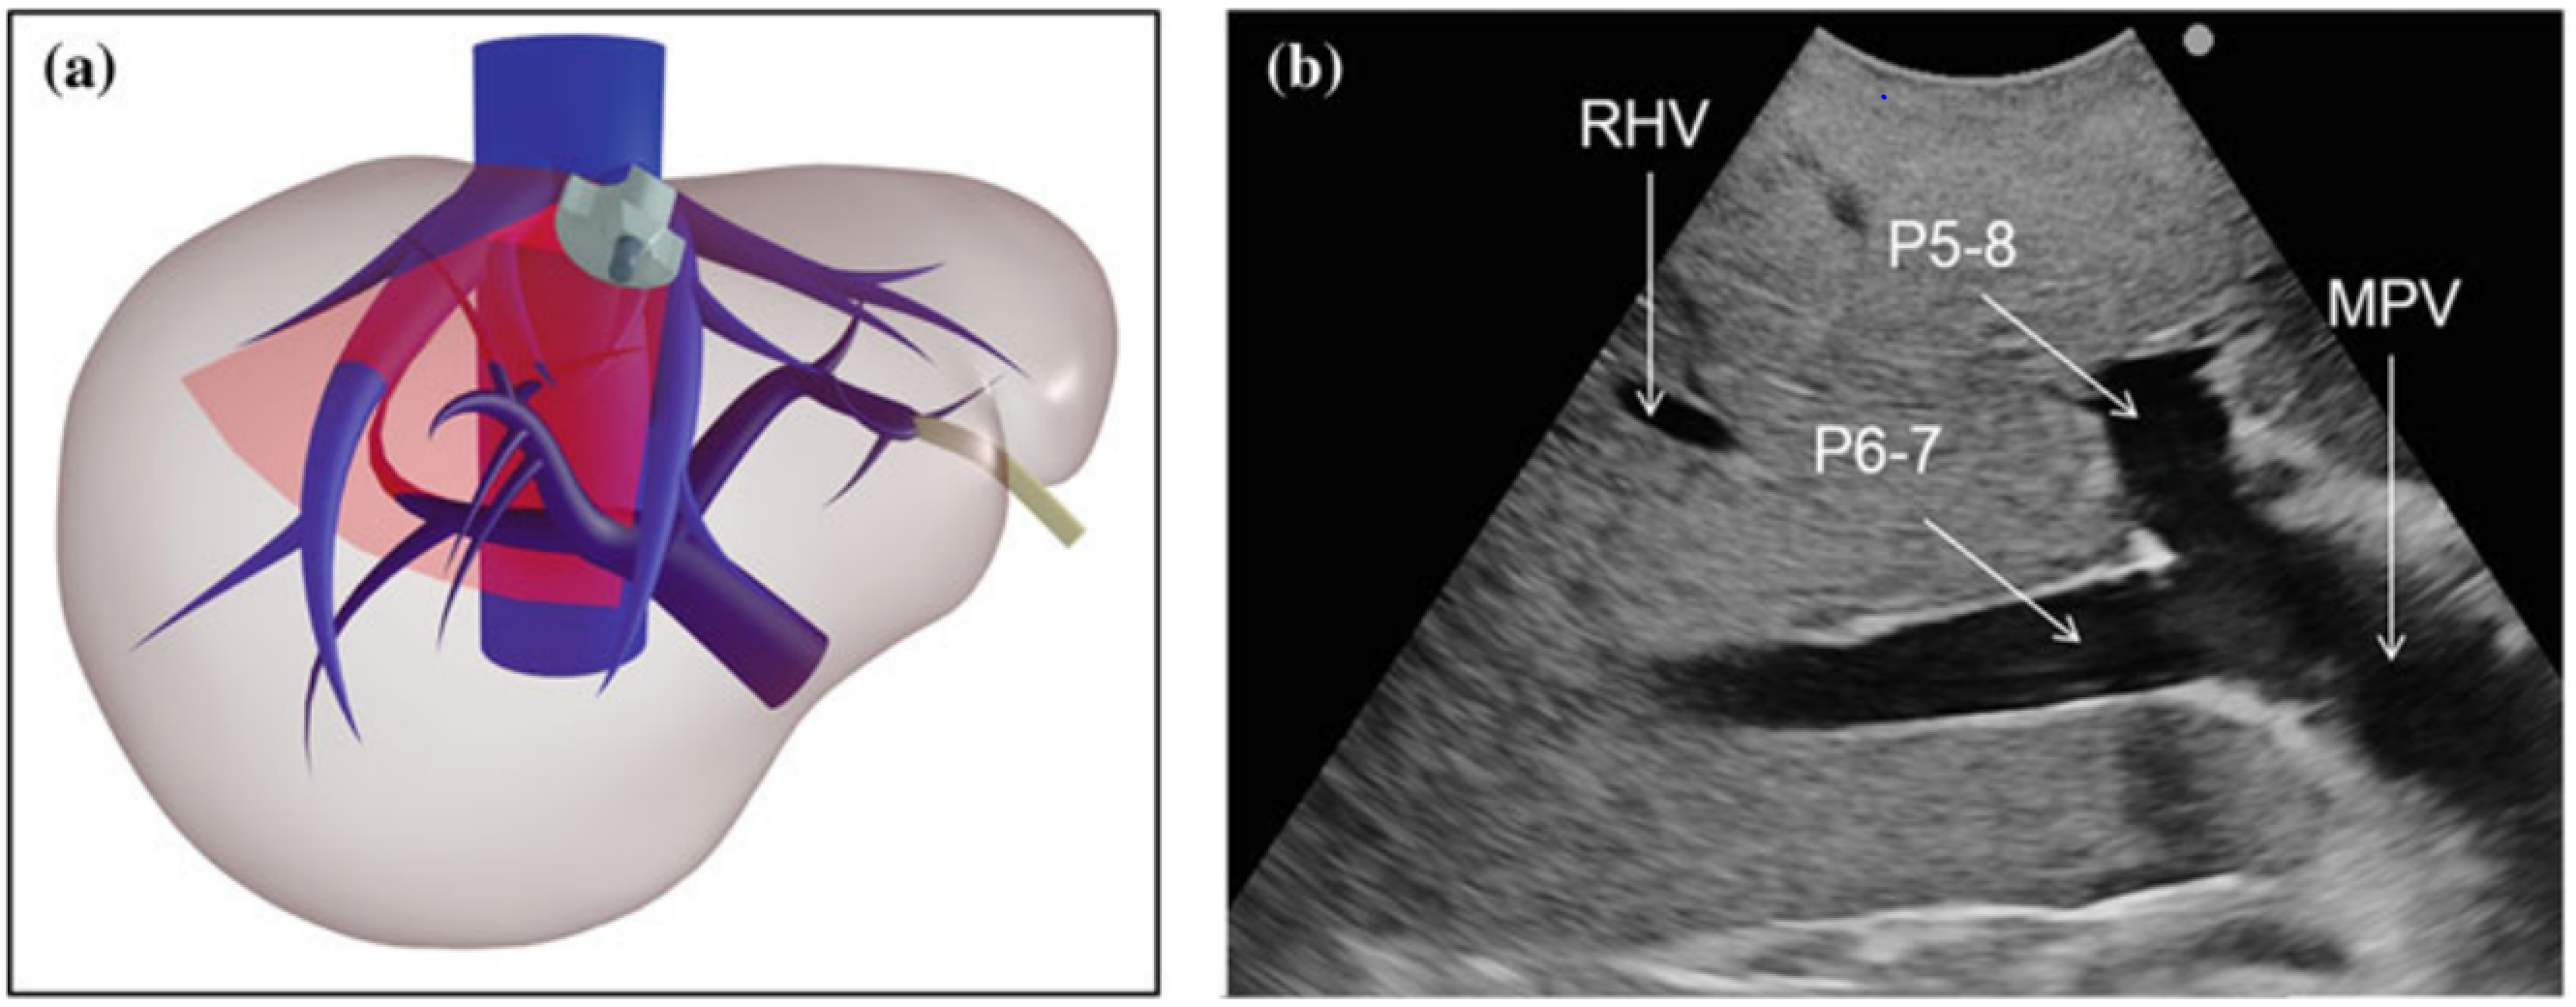
\includegraphics[width=\textwidth]{liverUS}
 \caption{ Left (a) ultrasound image plane in the liver. Right (b) intraoperative
   ultrasound image. One can see the right hepatic vein (RHV), the portal branch
   to segments 5 and 8 (P5-8) and the portal branch to segments 6 and 7 (P6-7) \cite{torzilli2014ultrasound}}
  \label{fig:liverUS}
\end{figure}

Ultrasound imaging works by the \textit{pulse-echo} principle. A short
ultrasound pulse is emitted from a transducer. The sound waves get
transmitted and reflected differently by different tissues. The reflected
 waves travel back into the transducer and are converted into an electrical
signal. After post-processing these signals become ultrasound images. 
The ultrasound measures the mechanical properties of the tissue. The tissues
have different acoustic impedance, which is the product of tissue density and
ultrasound speed in travelling through the tissue. The resolution of the
ultrasound images depends on the frequency of the ultrasonic waves. High
frequencies lead to higher resolution but lower penetration depth into the tissue because the
absorption of the sound energy increases with frequency too. Therefore the
useability to see deep structures is limited \cite{torzilli2014ultrasound}. 

In liver surgeries ultrasound is an important and established instrument.
Intraoperatively, the ultrasound is used on the liver surface directly,
therefore the penetration depth of the
ultrasound is optimal to represent the inner structures of the liver.
Registration methods based on 3D ultrasound reconstructed liver vessels 
exist but are not used in practice frequently \cite{lange2003vessel}. Ultrasound
is not harmful to health and therefore, can
be used as often as desired to navigate during a surgery.
% it is  
% Intraoperatively surgeons use ultrasound to localize the tumor as it gives
% advantages of reduced surgical time, complexity and radiation dosage.

\section{Navigation for liver resection surgeries}
\label{sec:navigationForLiverResections}
% \textcolor{green}{first, why is navigation needed, then how does it generally work
%   1) preoperative model or surgical plan 2) tracking 3) registration 4)
%   navigation visualization etc. then challenges especially in liver surgery and limitations}
It is a difficult task for inexperienced surgeons to orientate themselves within the liver during an operation.
From the outside of the liver it is not visible where the blood vessels are which they do not want to hurt.
Navigation can help surgeons to orient themselves precisely in organs during
operations.

% The actual intervention in computer assisted surgeries (CAS) is defined as
% surgical navigation.
A navigated operation differs in a few points from a non-navigated operation.
Because every patient's liver is different, a new 3D model of the liver has to
be created before surgery. This models are created from pre-operative 3D
computer tomography (CT) scan of the liver. Then, using this model, a surgical plan is made.
In contrast to a conventional operation, a navigation system is located in the
operating theatre and the surgical instruments can be tracked by it. Therefore special instruments are used. These
instruments have the ability to be tracked by the naviagation system. Depending
on the tracking technology used by the navigation system, the tools are different.
In order to also track the liver, the created model is registered to the anatomy
of the patient. Finally the orientation and position
of the instruments in relation to the patient's anatomy is visualized on a
monitor in the operating room. The surgeon can see what he does on the
monitor and uses the system to navigate the location and position of its
instruments. This is specialy then useful when the tip of the instrument is not
actually visible for the suergeon. While the tool tip is not visible, the
surgeon has to trust the navigation system. The accuracy of a recently developed system 
was 4.5 mm $\pm$3.6 mm averaged over nine surgeries \cite{peterhans2011navigation}.
Current research tries to compensate for deformations of the liver between the CT
scan to the actual shape of the liver during the surgery \cite{clements2017deformation}
\cite{clements2015validation}. 
\subsection{Creation of preoperative 3D-models}
Several steps are necessary to create a preoperative model. First the 
CT scan is done. This leads to representations of the liver on several 2D images parallel
to each other, filling a square volume with voxels. From this data the liver and
its inner structures are manually segmented and merged to a 3D model (Figure \ref{fig:MeVisExample}). This is very
time consuming and therefore expensive \cite{numminen2005preoperative}.
Nevertheless the resulting models are very detailed and accurate.
\begin{figure}[H]
  \centering
 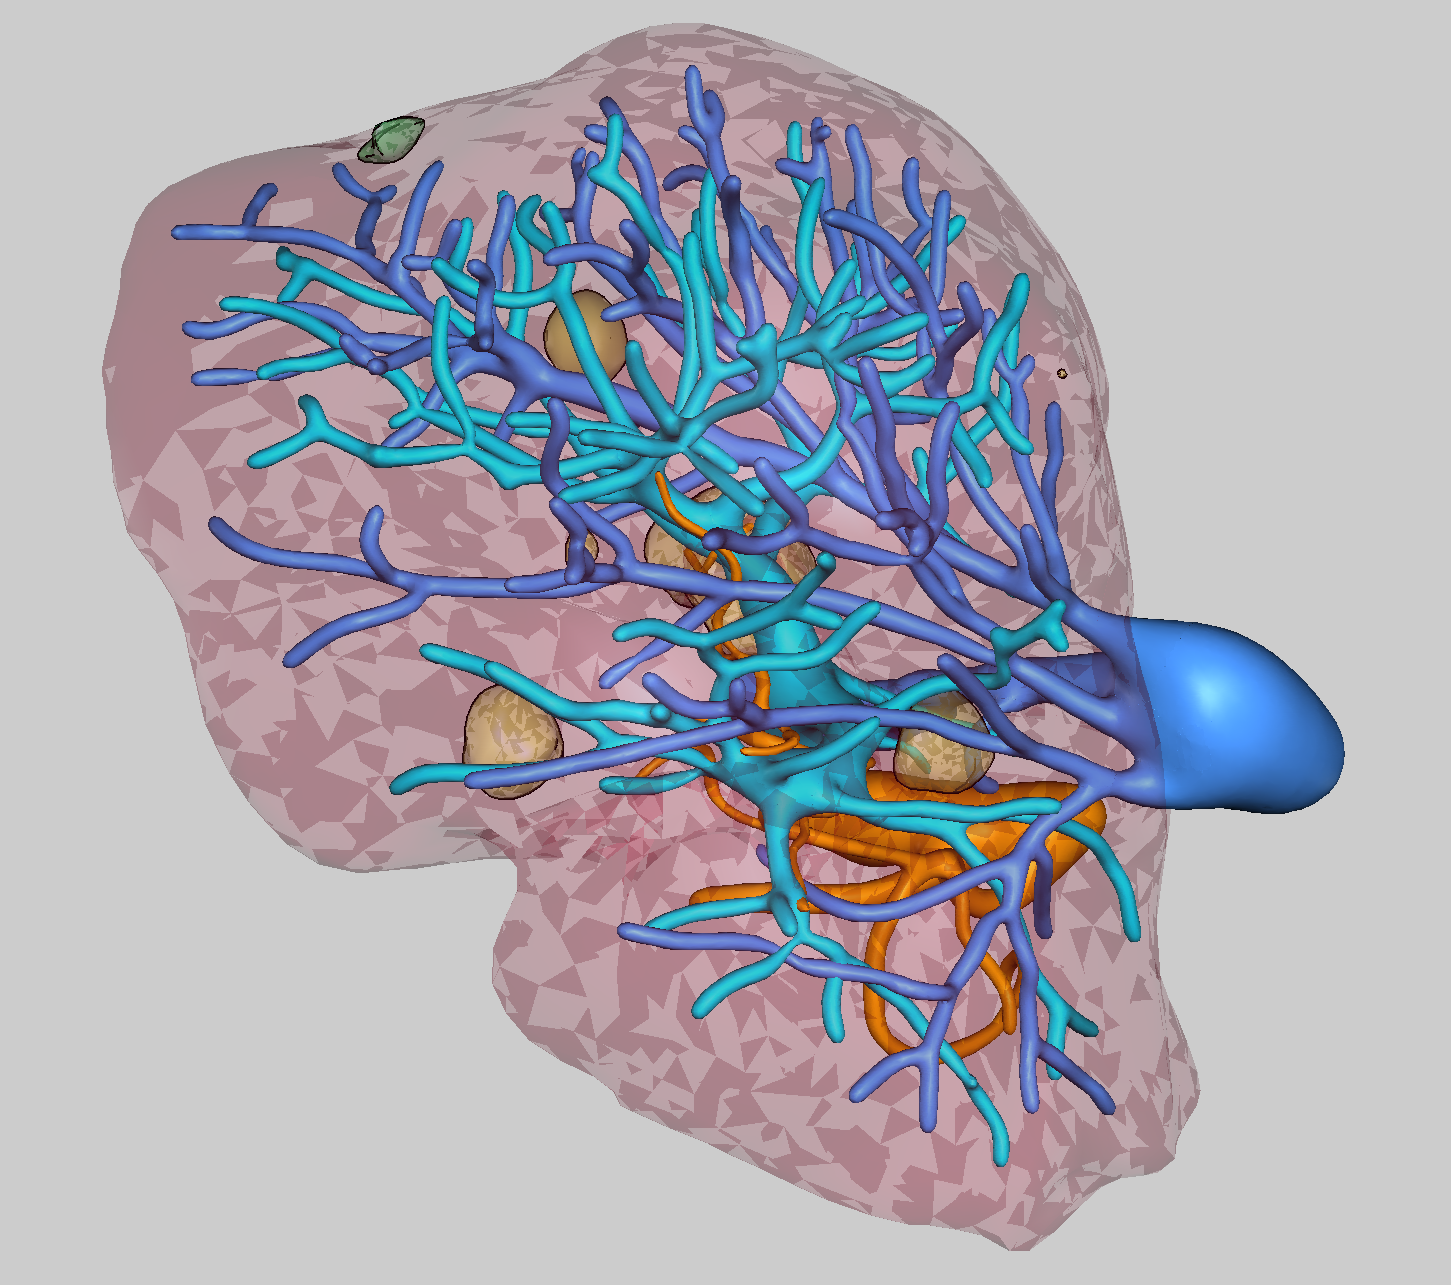
\includegraphics[width=0.6\textwidth]{MeVisExample}
 \caption{Example of a preoperative 3D model created by MeVis}%DK patient
  \label{fig:MeVisExample}
\end{figure}

\subsection{Registration}
Patient registration is a concept to correlate the reference coordinate system
of a virtual 3D data set with that of a patient. First, the 3D data set has to
be gathered. This is often done by CT or magnetic resonance imaging (MRI) scan of the patients anatomy to be
operated on. Secondly, finding of the transformation between the patient's
reference coordinate system and the virtual data set. During the surgery the patient is similarly
tracked as the instruments (see section \ref{sec:navigationForLiverResections}).
In this way, the patient has his own coordinate system. From here many different
methods exist to align the virtal data to the real anatomy.
Discrete landmarks, surface scans and
volumetric sonography scans are just a few of the approaches that can be
used to achieve precise alignment of the data with the
surgical site \cite{banz2016intraoperative}. Ultrasound based registration
methods in liver surgeries are further discussed in section
\ref{sec:ultrasoundBasedRegistration}.

\subsection{Tracking modalities}
To track surgical instruments and patient's anatomy (define the position and
orientation in real time) during naviagated surgery a tracking system is needed.
Tracking can be done by different technologies. The most used two tracking
modalities are optical and electromagnetic tracking.   

\subsubsection{Optical tracking}
Optical tracking is the most used tracking modality in naviagated liver
surgeries. Passive markers (spherical, retro-reflective that reflect infrared
light) or active markers (infrared-emitting markers that are activated by an
electrical signal) \cite{wiles2004accuracy} are attached to the objects that
need to be tracked. A tracking camera is then emitting infrared light by illuminators
on the position sensor (only for passive markers). The position sensor
determines the position and orientation of the tracked instruments based on the
information it receives from those markers \cite{noauthor_polaris_nodate}.  

\subsubsection{Electromagnetic tracking}
Electromagnetic (EM) tracking is a modality which uses small coils as markers
integrated in surgical instruments. A plate below the patient is used to
generate an electromagnetic field which defines the workspace of the tracking
system. The position and orientation of the tools in this workspace can be
estimated by measuring the signals received by the small coils. This tracking technology does not rely on a
line-of-sight and is therefore used in cases where the tracked instruments are
inside the patients body.  
\endinput
%%% Local Variables:
%%% TeX-master: "MscThesis"
%%% End: